\documentclass[12pt,a4paper]{ctexart}
\usepackage[a4paper,left=2.6cm,right=2.6cm,top=2.8cm,bottom=2.8cm]{geometry}
\usepackage{graphicx}
\usepackage{booktabs}
\usepackage{tabularx}
\usepackage{longtable}
\usepackage{array}
\usepackage{multirow}
\usepackage{amsmath,amssymb}
\usepackage{hyperref}
\usepackage{caption}
\usepackage{float}
\usepackage{enumitem}
\usepackage{setspace}
\usepackage{makecell}
\usepackage{ragged2e}
\hypersetup{colorlinks=true,linkcolor=black,citecolor=black,urlcolor=black}
\setlength{\parindent}{2em}
\setlength{\parskip}{0.3em}
\renewcommand{\arraystretch}{1.25}
% 让 tabularx 的 X 列使用 m{}，从而实现垂直居中
\renewcommand{\tabularxcolumn}[1]{m{#1}}
% 短文本/数字列：水平居中 + 垂直居中
\newcolumntype{C}[1]{>{\centering\arraybackslash}m{#1}}
% 长文本固定列：左对齐 + 垂直居中，避免中文长段强制居中导致视觉发散
\newcolumntype{L}[1]{>{\RaggedRight\arraybackslash}m{#1}}
% tabularx 自适应长文本列：左对齐 + 垂直居中
\newcolumntype{Y}{>{\RaggedRight\arraybackslash}X}
\captionsetup{font=small,labelsep=quad}
\onehalfspacing

\begin{document}
% =========================
% 作业报告封面页
% =========================
\begin{titlepage}
    \centering

    \vspace*{1.5cm}

    {\zihao{-1}\heiti 北京邮电大学\par}

    \vspace{0.8cm}

    {\zihao{2}\heiti 《信息安全管理》课程大作业\par}

    \vspace{2.5cm}

    {\zihao{1}\heiti AI辅助开发过程中的安全管理实践报告\par}

    \vspace{3.2cm}

    \begin{center}
    \renewcommand{\arraystretch}{1.8}
    \zihao{4}
    \begin{tabular}{>{\heiti}r p{8cm}}
        学生姓名： & \makebox[8cm][l]{\hspace{2.5cm}陈柯睿} \\ \cline{2-2}
        学\hspace{2em}号： & \makebox[8cm][l]{\hspace{2.0cm}2023211478} \\ \cline{2-2}
        专业班级： & \makebox[8cm][l]{\hspace{2.0cm}2023211802} \\ \cline{2-2}
        学\hspace{2em}院： & \makebox[8cm][l]{\hspace{1.4cm}网络空间安全学院} \\ \cline{2-2}
        指导老师： & \makebox[8cm][l]{\hspace{2.7cm}郭燕慧} \\ \cline{2-2}
    \end{tabular}
    \end{center}

    \vfill

    {\zihao{4} 北京邮电大学\par}
    \vspace{0.5cm}
    {\zihao{4} \today\par}

\end{titlepage}

\tableofcontents
\newpage

\section{作业背景与完成概况}

本次作业要求在前两次作业仓库基础上，使用 AI 编程工具完成一个新模块或对现有模块进行实质性安全修改，并在开发过程中落实风险识别、安全约束表达、AI 生成结果审查、问题整改与验证等安全管理要求。

本次选择的模块为仓库中的“桌面宠物待办清单”：

\begin{verbatim}
成员代码/桌面宠物代办清单-陈柯睿/
\end{verbatim}

该模块是一个基于 Flask 的轻量级待办应用，前端通过 \texttt{fetch} 调用后端 JSON 接口，后端原本将待办数据保存到本地 JSON 文件中。原始版本中，待办数据接口无需身份验证即可访问，存在未授权读取和修改待办数据的风险。本次作业将其作为安全加固对象，新增用户注册/登录模块，为现有接口增加权限校验逻辑，将待办数据按用户隔离保存，并新增一个必须身份验证才能访问的账号概览接口。

\begin{table}[H]
    \centering
    \caption{本次作业基本信息}
    \begin{tabularx}{\textwidth}{C{3.2cm}Y}
        \toprule
        项目 & 内容 \\
        \midrule
        仓库名称 & \texttt{Information\_Security\_Management} \\
        修改分支 & \texttt{feature/pet-todo-session-auth} \\
        Commit Message & \texttt{feat: 为桌面宠物待办增加用户认证} \\
        Commit Hash & 以 PR 最新提交为准 \\
        负责环节 & 安全整改 / 功能加固 / 过程文档整理 \\
        涉及模块 & 桌面宠物待办清单 \\
        主要安全点 & 用户注册登录、密码哈希、接口权限校验、用户数据隔离、错误响应控制 \\
        \bottomrule
    \end{tabularx}
\end{table}

\section{模块修改说明}

\subsection{修改前的问题}

修改前，桌面宠物待办清单的核心接口包括：

\begin{itemize}[leftmargin=2.5em]
    \item \texttt{GET /api/state}：获取当前待办状态；
    \item \texttt{POST /api/todos}：新增待办；
    \item \texttt{PATCH /api/todos/<todo\_id>}：更新待办完成状态；
    \item \texttt{DELETE /api/todos/<todo\_id>}：删除待办；
    \item \texttt{POST /api/todos/clear-done}：清除已完成待办；
    \item \texttt{POST /api/pet/pat}：获取宠物反馈。
\end{itemize}

这些接口直接读写本地待办数据，但原实现没有身份验证或权限判断。如果 Flask 服务被暴露到局域网或公网，其他用户可以绕过页面交互，直接请求接口读取或篡改待办数据。同时，原模块没有用户概念，无法区分不同用户的数据归属。

\subsection{修改后的功能}

本次修改为该模块增加了基于 Flask Session 的注册/登录模块。新增接口如下：

\begin{table}[H]
    \centering
    \caption{新增认证相关接口}
    \begin{tabularx}{\textwidth}{C{4.2cm}C{2.2cm}Y}
        \toprule
        接口 & 方法 & 作用 \\
        \midrule
        \texttt{/api/session} & GET & 查询当前登录状态和用户名 \\
        \texttt{/api/register} & POST & 注册新用户，密码经 PBKDF2 哈希后保存 \\
        \texttt{/api/login} & POST & 校验用户名和密码，登录成功后建立会话 \\
        \texttt{/api/logout} & POST & 清除当前会话，退出登录 \\
        \texttt{/api/account/summary} & GET & 登录后查看当前账号和待办概览 \\
        \bottomrule
    \end{tabularx}
\end{table}

同时，所有涉及待办数据读取或修改的接口均添加 \texttt{@login\_required} 装饰器，未登录访问时统一返回 \texttt{401} 状态码。用户密码不明文保存，而是使用随机盐和 PBKDF2 哈希后写入 \texttt{data/users.json}；待办状态按用户 ID 保存到 \texttt{data/user-states/}，从数据存储层降低横向越权风险。

\subsection{运行截图与修改思路说明}

本地运行桌面宠物待办清单后，页面首先展示新增的注册/登录入口，如图~\ref{fig:pet-todo-login} 所示。该截图对应本次修改后的前端初始状态：用户未登录时只能看到认证面板，不能直接看到待办列表或触发待办数据接口。

\begin{figure}[H]
    \centering
    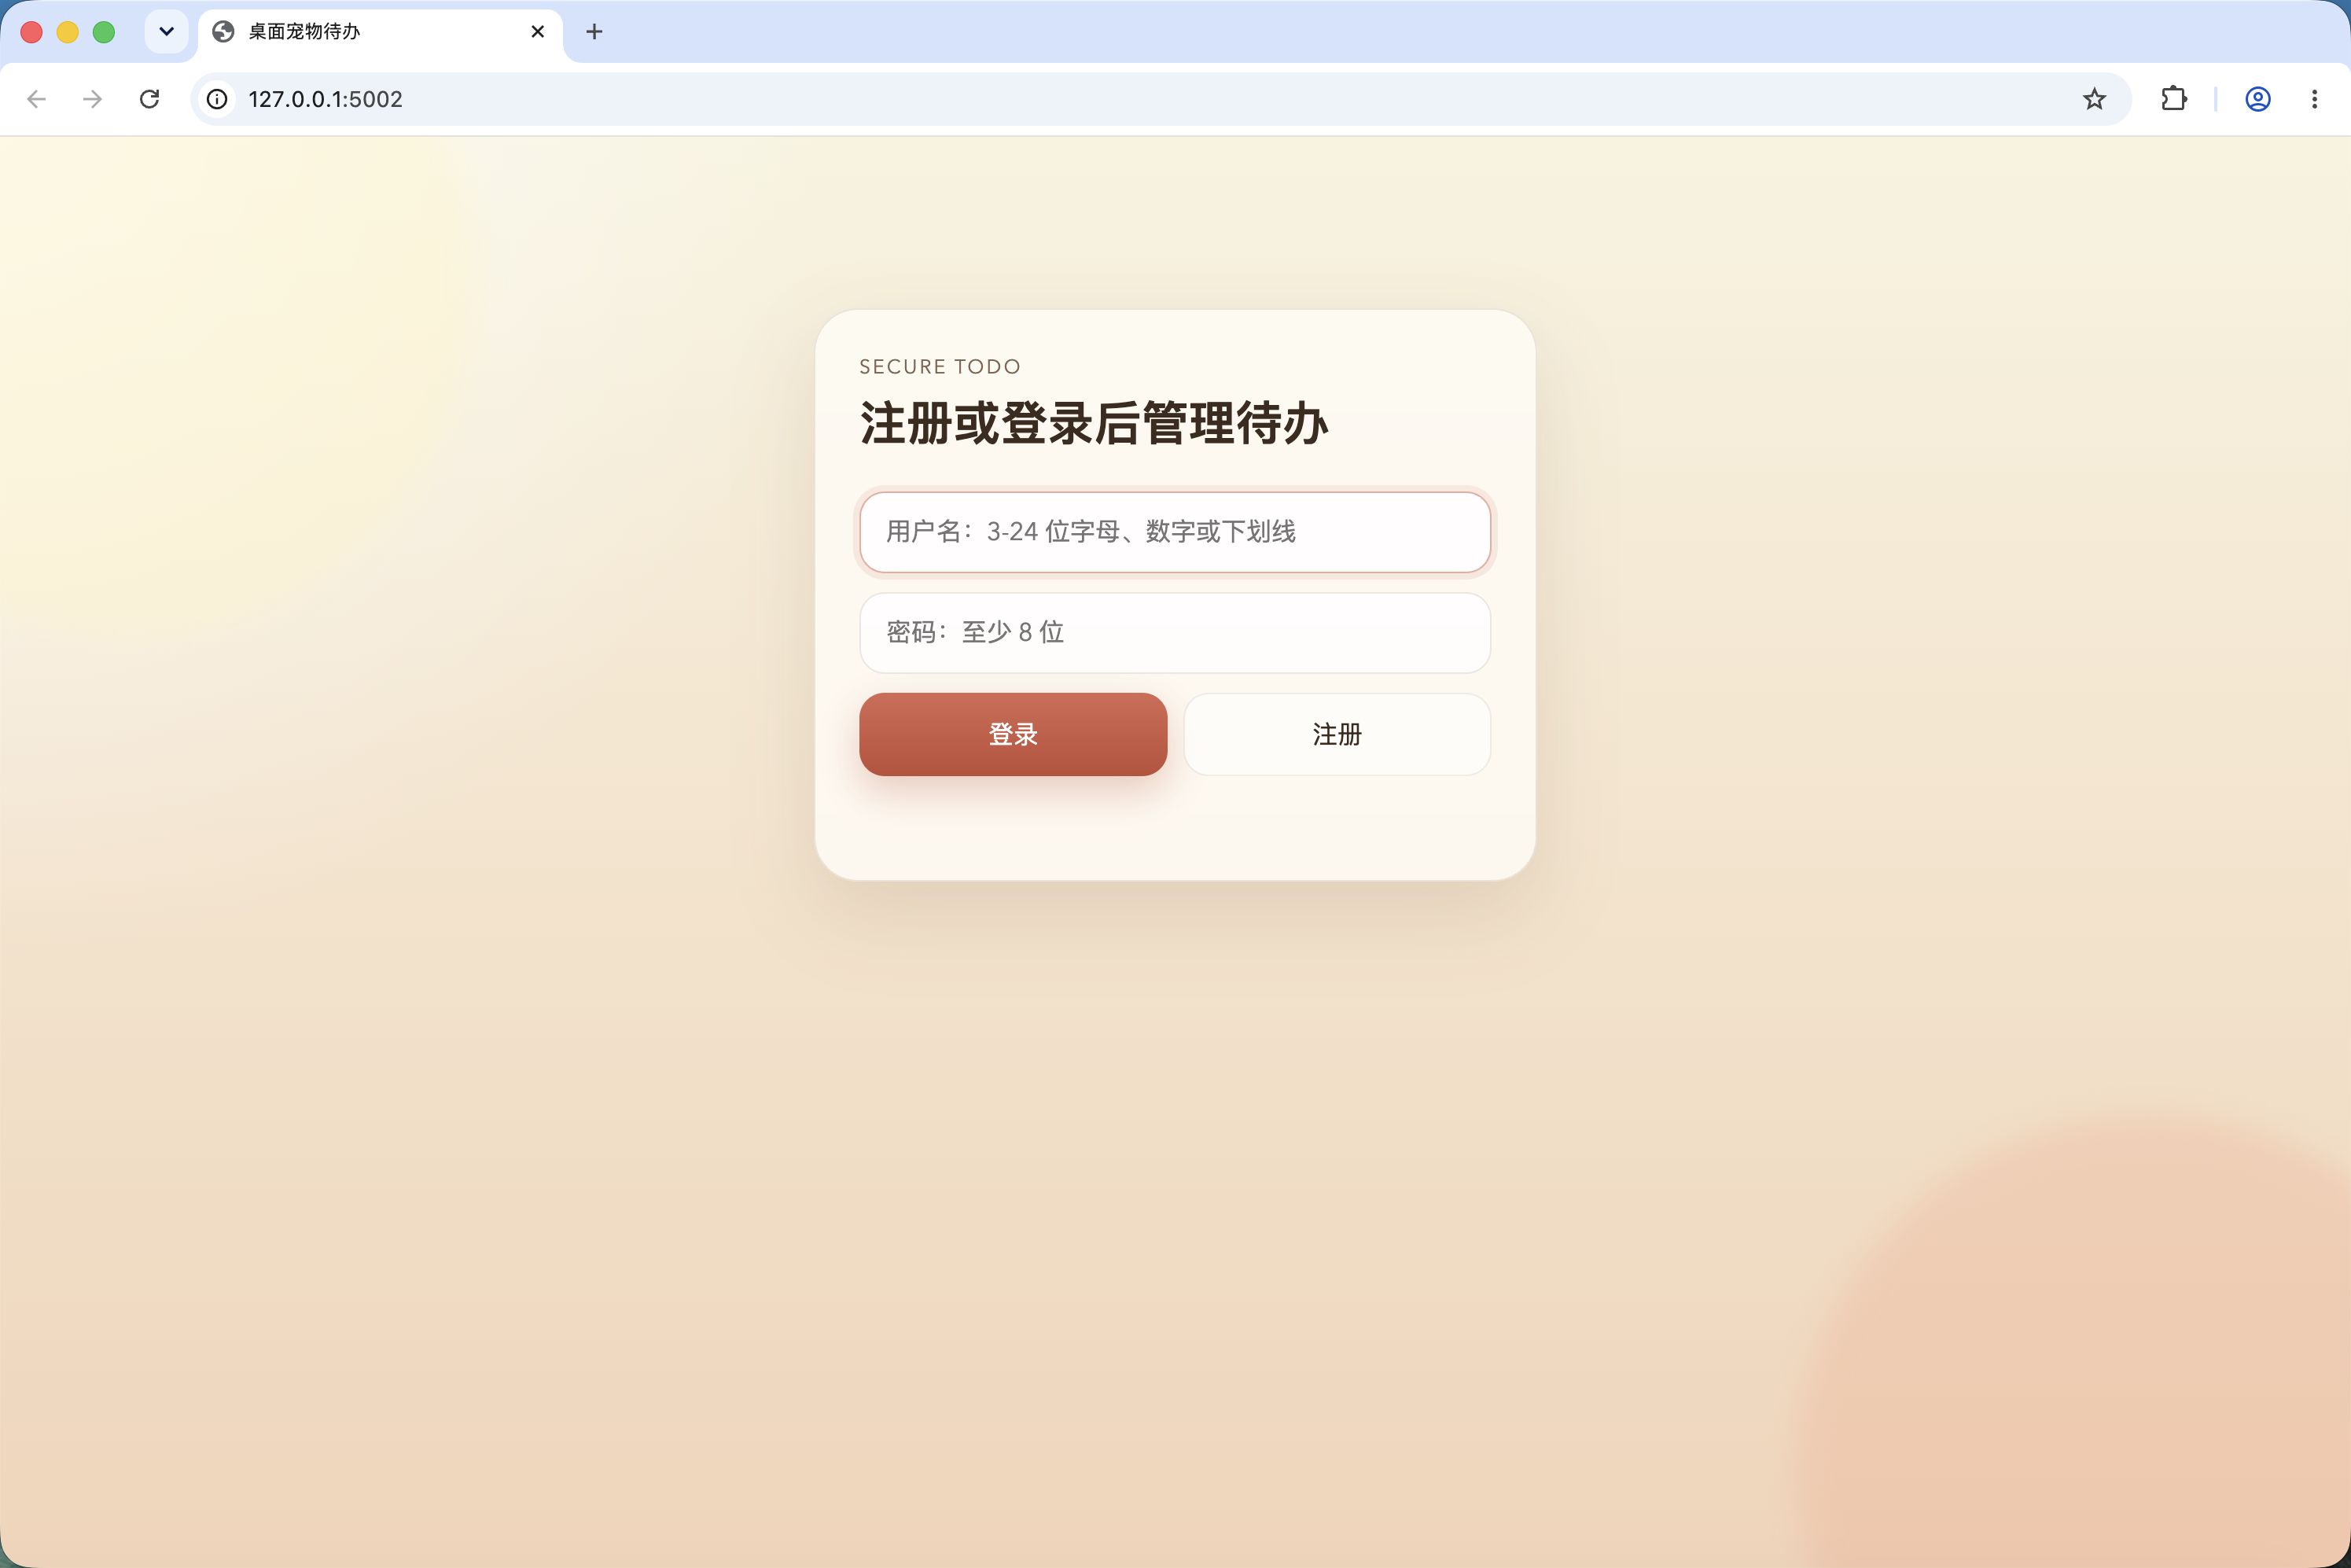
\includegraphics[width=0.95\textwidth]{assets/pet-todo-login.png}
    \caption{桌面宠物待办清单新增注册/登录模块后的运行界面}
    \label{fig:pet-todo-login}
\end{figure}

从图~\ref{fig:pet-todo-login} 可以看出，本次修改不是简单地在 README 中补充说明，而是将“先注册或登录、再访问数据”的安全控制显式加入到应用交互流程中。前端修改集中在 \texttt{templates/index.html}、\texttt{static/script.js} 和 \texttt{static/styles.css}：新增用户名和密码输入、注册按钮、登录状态切换逻辑和对应样式。后端修改集中在 \texttt{app.py}：新增 \texttt{/api/register}、\texttt{/api/session}、\texttt{/api/login}、\texttt{/api/logout} 和 \texttt{/api/account/summary}，并用 \texttt{login\_required} 装饰器保护待办数据接口。这样即使攻击者绕过前端页面直接请求接口，后端仍会返回 \texttt{401}，安全控制不会只停留在页面展示层。

\section{风险识别}

在编写 Prompt 和修改代码之前，先对选定模块进行风险识别，明确其中涉及的敏感操作和潜在安全问题。

\subsection{敏感操作分析}

\begin{longtable}{C{4cm}Y}
    \caption{敏感操作与风险点分析}\\
    \toprule
    敏感操作 & 风险说明 \\
    \midrule
    \endfirsthead
    \toprule
    敏感操作 & 风险说明 \\
    \midrule
    \endhead
    读取待办数据 & 待办内容可能包含个人计划、学习安排或其他隐私信息，未经授权读取会造成信息泄露。 \\
    新增待办 & 未授权用户可以写入无关内容，污染本地数据。 \\
    修改完成状态 & 未授权用户可以改变任务完成情况，破坏数据完整性。 \\
    删除待办 & 未授权用户可以删除任务，造成数据丢失。 \\
    清除已完成待办 & 批量删除操作影响范围更大，需要登录后才能执行。 \\
    用户注册与登录 & 涉及用户名、密码校验和会话建立，如果处理不当会造成凭据泄露或账号枚举。 \\
    账号概览查询 & 该接口汇总当前用户任务数量和成长状态，必须确认访问者身份。 \\
    本地 JSON 文件读写 & 文件中保存用户凭据哈希和任务状态，如果缺少用户隔离会导致横向越权。 \\
    \bottomrule
\end{longtable}

\subsection{识别出的主要风险}

\begin{enumerate}[leftmargin=2.5em]
    \item \textbf{未授权访问风险}：原接口不需要登录即可读取和修改待办数据，缺少基本身份认证。
    \item \textbf{明文密码风险}：新增注册登录后，如果直接保存明文密码，会造成严重凭据泄露风险。
    \item \textbf{横向越权风险}：如果多个用户仍然共享同一个待办状态文件，就可能互相读取或修改任务。
    \item \textbf{错误响应泄露风险}：登录失败或未授权访问时，不应返回用户是否存在、文件路径或异常堆栈等内部细节。
\end{enumerate}

风险识别记录已保存到：

\begin{verbatim}
docs/risk-analysis.md
\end{verbatim}

\section{安全约束表达}

根据风险识别结果，将安全要求转化为 AI 交互中的明确约束，避免 AI 只实现表面功能而忽略安全边界。

\subsection{约束文档}

本次编写了项目约束文档 \texttt{docs/constraint-doc.md}。其中规定：

\begin{itemize}[leftmargin=2.5em]
    \item 必须新增用户注册和登录接口；
    \item 密码不能明文保存，必须使用随机盐和密码哈希；
    \item 未登录访问待办数据接口必须返回 \texttt{401}；
    \item 登录接口不得泄露用户名是否存在、文件路径或异常堆栈；
    \item 不同用户的待办数据必须隔离保存；
    \item 前端不得将密码写入 \texttt{localStorage} 或 \texttt{sessionStorage}；
    \item 安全控制必须落在后端接口层，不能只依赖前端隐藏按钮或页面；
    \item 禁止硬编码默认管理员密码；
    \item 禁止提交 \texttt{.env}、密钥、证书、本地数据库等敏感文件。
\end{itemize}

\subsection{结构化 Prompt}

AI 交互中使用的核心 Prompt 按“背景说明 / 任务范围 / 约束条件 / 禁止行为”的结构组织。关键内容如下：

\begin{verbatim}
为 Flask 桌面宠物待办模块实现完整安全加固。
必须完成：
1. 新增用户注册/登录模块。
2. 为现有待办接口新增权限校验逻辑。
3. 修复原模块接口公开访问的问题，写出安全加固版本。
4. 新增一个必须登录才能访问的功能接口。

约束：
- 密码不能明文保存，不能硬编码默认账号。
- 密码需要使用随机盐和安全哈希。
- 未登录访问受保护接口返回 401。
- 登录失败不能暴露用户名是否存在。
- 不同用户的待办数据必须隔离。
- 前端不能把密码写入 localStorage 或 sessionStorage。
- 安全控制必须在后端接口层实现。
\end{verbatim}

Prompt 记录已保存到：

\begin{verbatim}
docs/prompt-records.md
\end{verbatim}

\section{AI 生成结果检查与安全审查}

\subsection{对照 Prompt 的功能检查}

AI 生成代码后，首先对照 Prompt 检查功能是否实际实现，安全约束是否落实到代码逻辑中，而不是仅停留在注释或文档中。

\begin{table}[H]
    \centering
    \caption{Prompt 对照检查结果}
    \begin{tabularx}{\textwidth}{L{5cm}C{2cm}Y}
        \toprule
        检查项 & 结果 & 说明 \\
        \midrule
        是否新增注册接口 & 通过 & 新增 \texttt{/api/register} \\
        是否新增登录接口 & 通过 & 新增 \texttt{/api/login}、\texttt{/api/logout}、\texttt{/api/session} \\
        待办数据接口是否需要登录 & 通过 & 核心接口均添加 \texttt{@login\_required} \\
        是否新增受保护功能接口 & 通过 & 新增 \texttt{/api/account/summary} \\
        是否避免明文密码 & 通过 & 使用 PBKDF2、随机盐和迭代次数保存密码哈希 \\
        前端是否持久化密码 & 通过 & 密码只在注册/登录请求中提交，不写入浏览器持久存储 \\
        未登录是否返回 401 & 通过 & 由 \texttt{login\_required} 统一处理 \\
        原有待办功能是否保留 & 通过 & 登录后新增、完成、删除等主流程可用 \\
        \bottomrule
    \end{tabularx}
\end{table}

\subsection{人工安全审查}

第二层检查重点关注认证授权分层、最小权限、错误响应等业务逻辑。

\begin{table}[H]
    \centering
    \caption{人工安全审查结果}
    \begin{tabularx}{\textwidth}{L{5cm}C{2cm}Y}
        \toprule
        检查项 & 结果 & 说明 \\
        \midrule
        认证控制是否在后端 & 通过 & 前端隐藏界面只是体验优化，真正拦截在 Flask API 层 \\
        最小权限原则 & 通过 & 登录用户只能访问自己的待办状态和账号概览 \\
        用户数据是否隔离 & 通过 & 待办状态按用户 ID 保存到 \texttt{data/user-states/} \\
        错误响应是否过度暴露 & 通过 & 登录失败统一返回“用户名或密码不正确” \\
        敏感配置是否进入仓库 & 通过 & 未提交真实密码、密钥或 \texttt{.env} \\
        Session Cookie 是否有基础安全属性 & 通过 & 显式配置 \texttt{HttpOnly} 和 \texttt{SameSite=Lax} \\
        调试模式是否默认关闭 & 通过 & 只有设置 \texttt{FLASK\_DEBUG=1} 时才开启 \\
        \bottomrule
    \end{tabularx}
\end{table}

安全审查清单已保存到：

\begin{verbatim}
docs/security-checklist.md
\end{verbatim}

\section{问题整改与实现细节}

\subsection{后端整改}

后端主要修改文件为：

\begin{verbatim}
成员代码/桌面宠物代办清单-陈柯睿/app.py
\end{verbatim}

关键整改包括：

\begin{enumerate}[leftmargin=2.5em]
    \item 新增 \texttt{/api/register}，实现用户注册模块；
    \item 新增 \texttt{/api/login}、\texttt{/api/logout} 和 \texttt{/api/session}，实现登录、登出和会话状态查询；
    \item 新增 \texttt{/api/account/summary}，作为必须身份验证才能访问的功能接口；
    \item 使用 \texttt{hashlib.pbkdf2\_hmac()}、随机盐和迭代次数保存密码哈希，避免明文密码；
    \item 新增 \texttt{is\_authenticated()}，判断当前 Flask Session 是否已登录；
    \item 新增 \texttt{login\_required} 装饰器，对受保护接口统一拦截；
    \item 登录时使用 \texttt{hmac.compare\_digest()} 比较密码哈希，避免普通字符串比较可能产生的细节泄露；
    \item 登录成功后写入 \texttt{session}，登出时清除 \texttt{session}；
    \item 将待办状态按用户 ID 保存到 \texttt{data/user-states/}，避免不同用户共享同一份状态；
    \item 显式配置 \texttt{SESSION\_COOKIE\_HTTPONLY=True} 和 \texttt{SESSION\_COOKIE\_SAMESITE="Lax"}；
    \item 保持 Flask debug 模式默认关闭。
\end{enumerate}

\subsection{前端整改}

前端主要修改文件为：

\begin{verbatim}
成员代码/桌面宠物代办清单-陈柯睿/templates/index.html
成员代码/桌面宠物代办清单-陈柯睿/static/script.js
成员代码/桌面宠物代办清单-陈柯睿/static/styles.css
\end{verbatim}

关键整改包括：

\begin{itemize}[leftmargin=2.5em]
    \item 新增注册/登录面板，用户未登录时不展示待办主界面；
    \item 页面加载时先请求 \texttt{/api/session} 判断登录状态；
    \item 注册和登录时提交用户名与密码，不在浏览器持久化保存密码；
    \item 登录成功后再加载 \texttt{/api/state}；
    \item 登录后请求 \texttt{/api/account/summary} 展示当前用户名和等级；
    \item 新增退出登录按钮，调用 \texttt{/api/logout} 清除会话；
    \item 当接口返回 \texttt{401} 时，前端自动切回登录界面。
\end{itemize}

\subsection{文档整改}

README 中补充了新的运行方式、安全说明和数据存储说明。项目现在直接启动即可，首次使用时在页面中注册账号：

\begin{verbatim}
python app.py
\end{verbatim}

同时补充说明：密码不会明文保存，后端使用 PBKDF2 和随机盐保存密码哈希；未登录请求待办接口会返回 \texttt{401}；用户待办数据按用户 ID 隔离保存。

整改说明已保存到：

\begin{verbatim}
docs/fix-report.md
\end{verbatim}

\section{验证过程}

\subsection{静态检查}

完成修改后，首先运行 Python 语法检查：

\begin{verbatim}
python3 -m py_compile 成员代码/桌面宠物代办清单-陈柯睿/app.py
\end{verbatim}

检查结果：通过。

随后运行 Git 空白与格式检查：

\begin{verbatim}
git diff --check
\end{verbatim}

检查结果：通过。

\subsection{接口级验证}

使用 Flask test client 对核心认证流程和待办主流程进行冒烟测试，覆盖以下场景：

\begin{itemize}[leftmargin=2.5em]
    \item 未登录访问 \texttt{/api/state} 返回 \texttt{401}；
    \item 未登录访问 \texttt{/api/account/summary} 返回 \texttt{401}；
    \item 注册用户成功；
    \item 重复用户名注册返回 \texttt{409}；
    \item 错误密码登录返回 \texttt{401}；
    \item 正确密码登录返回 \texttt{200}；
    \item 登录后访问 \texttt{/api/account/summary} 返回 \texttt{200}；
    \item 登录后可以新增待办；
    \item 登录后可以完成待办；
    \item 登录后可以删除待办；
    \item 第二个用户无法看到第一个用户的待办数据；
    \item 登出后再次访问 \texttt{/api/state} 返回 \texttt{401}。
\end{itemize}

接口级验证结果：全部通过。

\subsection{实际 HTTP 验证}

在本地启动服务后，使用 HTTP 请求进行实际验证：

\begin{verbatim}
GET  /              -> 200
GET  /api/state     -> 401
POST /api/register  -> 201
POST /api/login     -> 200
GET  /api/account/summary -> 200
GET  /api/state     -> 200
\end{verbatim}

上述结果说明：页面可以正常访问；未登录时无法读取待办数据；注册/登录成功后可以访问账号概览和待办状态。

其中，\texttt{GET /} 返回 \texttt{200} 对应图~\ref{fig:pet-todo-login} 中展示的注册/登录入口页面；\texttt{GET /api/state} 在未登录时返回 \texttt{401}，说明图中认证面板并非单纯的前端遮挡，而是与后端接口访问控制相配合。注册/登录成功后，\texttt{/api/account/summary} 和 \texttt{/api/state} 均可访问，说明认证通过后新增功能接口和原有待办功能都能正常工作。

扫描与验证报告已保存到：

\begin{verbatim}
reports/scan-report.md
reports/before-after-diff.md
\end{verbatim}

\section{PR 描述材料}

本次 Pull Request 可使用如下描述。

\subsection*{本次 PR 说明}

\begin{itemize}[leftmargin=2.5em]
    \item 负责的环节：整改 / 安全加固；
    \item 涉及的模块：桌面宠物待办清单；
    \item 修改分支：\texttt{feature/pet-todo-session-auth}；
    \item Commit Message：\texttt{feat: 为桌面宠物待办增加用户认证}。
\end{itemize}

\subsection*{识别的主要安全风险}

\begin{enumerate}[leftmargin=2.5em]
    \item 待办数据接口原本无需登录即可访问，存在未授权读取和篡改风险；
    \item 新增用户体系后，如果密码明文保存或用户数据不隔离，会造成凭据泄露和横向越权风险。
\end{enumerate}

\subsection*{安全约束如何进入 AI 交互}

在 Prompt 和约束文档中明确要求：必须新增用户注册/登录模块；待办数据接口必须登录后访问；密码不能明文保存；不同用户的待办数据必须隔离；认证控制必须在后端实现，不能只依赖前端隐藏页面；不得提交真实密码、密钥或 \texttt{.env} 文件。

\subsection*{审查发现的问题与处置}

审查发现原模块缺少身份认证控制，且没有用户数据边界。已新增注册、登录、登出、会话状态接口，并使用 \texttt{login\_required} 装饰器保护待办数据接口。新增 \texttt{/api/account/summary} 作为必须登录才能访问的功能接口。前端增加注册/登录面板，未登录时不会加载待办数据。

在接口级验证中还发现一个数据隔离问题：初始默认状态如果使用浅拷贝，会导致多个新用户共享同一个 \texttt{todos} 列表引用。该问题已整改为每次返回独立默认状态对象，并通过双用户测试确认第二个用户无法看到第一个用户的待办数据。

\subsection*{相关过程材料位置}

\begin{itemize}[leftmargin=2.5em]
    \item \texttt{docs/risk-analysis.md}
    \item \texttt{docs/constraint-doc.md}
    \item \texttt{docs/prompt-records.md}
    \item \texttt{docs/security-checklist.md}
    \item \texttt{docs/fix-report.md}
    \item \texttt{reports/scan-report.md}
    \item \texttt{reports/before-after-diff.md}
\end{itemize}

\section{总结}

本次作业围绕“AI 辅助开发过程中的安全管理实践”展开，没有停留在简单代码生成或文档补充，而是针对已有模块中实际存在的未授权访问问题进行了安全加固。通过风险识别、安全约束表达、AI 生成结果检查、人工安全审查、整改验证和过程留痕，形成了较完整的安全管理闭环。

从结果看，桌面宠物待办清单模块已经从“接口默认公开访问”改为“注册/登录后才能读取和修改自己的待办数据”。同时，密码使用 PBKDF2 和随机盐保存哈希，待办数据按用户 ID 隔离，并新增了登录后才能访问的账号概览接口。验证报告和前后对比文档说明，本次修改同时覆盖了用户注册/登录、现有接口权限校验、安全加固版本和新增受保护功能接口四项要求。该实现适合课程实验和本地演示场景，若后续部署到真实公网环境，还需要进一步增加 HTTPS、登录失败限速和更完善的审计日志。

\end{document}
